\subsection{Nativer Mobile Client}

Mit IP5 wurde bereits ein Client umgesetzt.
Dieser muss für IP6 migiert werden.
Hier wird beschrieben, wie die bestehenden Anforderungen mit dem nativen client umgesetzt werden können.

\subsubsection{Benutzeroberfläche}

Die Ansichten zur Anmeldung und Zimmerauswahl werden analog zum bestehenden Mobile Client umgesetzt.
Die Login Seite beinhaltet einen kurzen Willkommenstext und ein Logo für Praxisruf.
Darunter findet sich ein einfaches Formular zur Eingabe von Benutzername und Passwort.

\begin{figure}[h]
    \centering
    \begin{minipage}[b]{0.4\textwidth}
        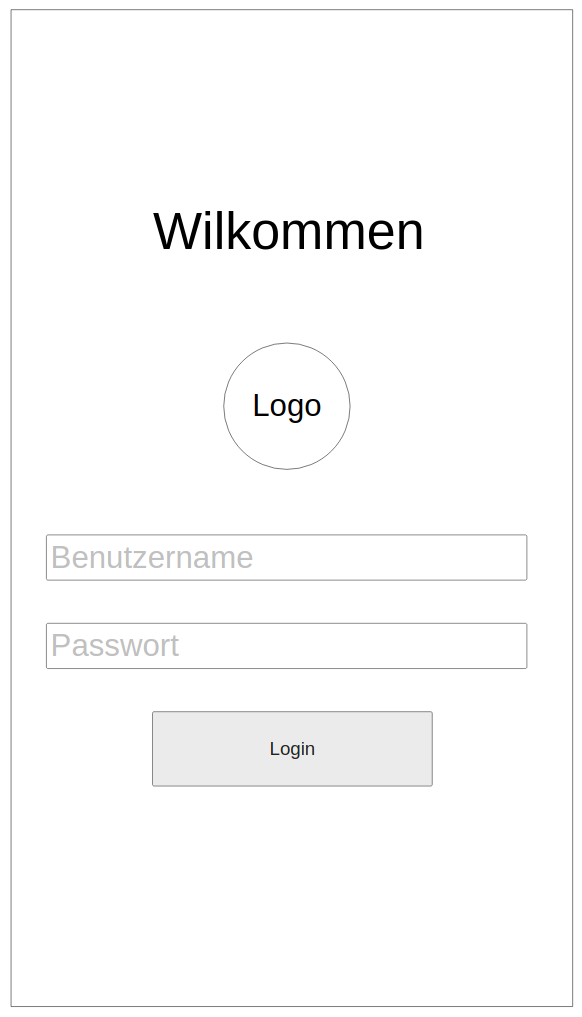
\includegraphics[width=\textwidth]{/home/joshua/FHNW/dev/IP6/IP6_Bachelorarbeit_Bericht_Cloudbasiertes_Praxisrufsystem/src/graphics/mockups/mockup_login}
        \caption{Mockup Login}
    \end{minipage}
    \hfill
    \begin{minipage}[b]{0.4\textwidth}
        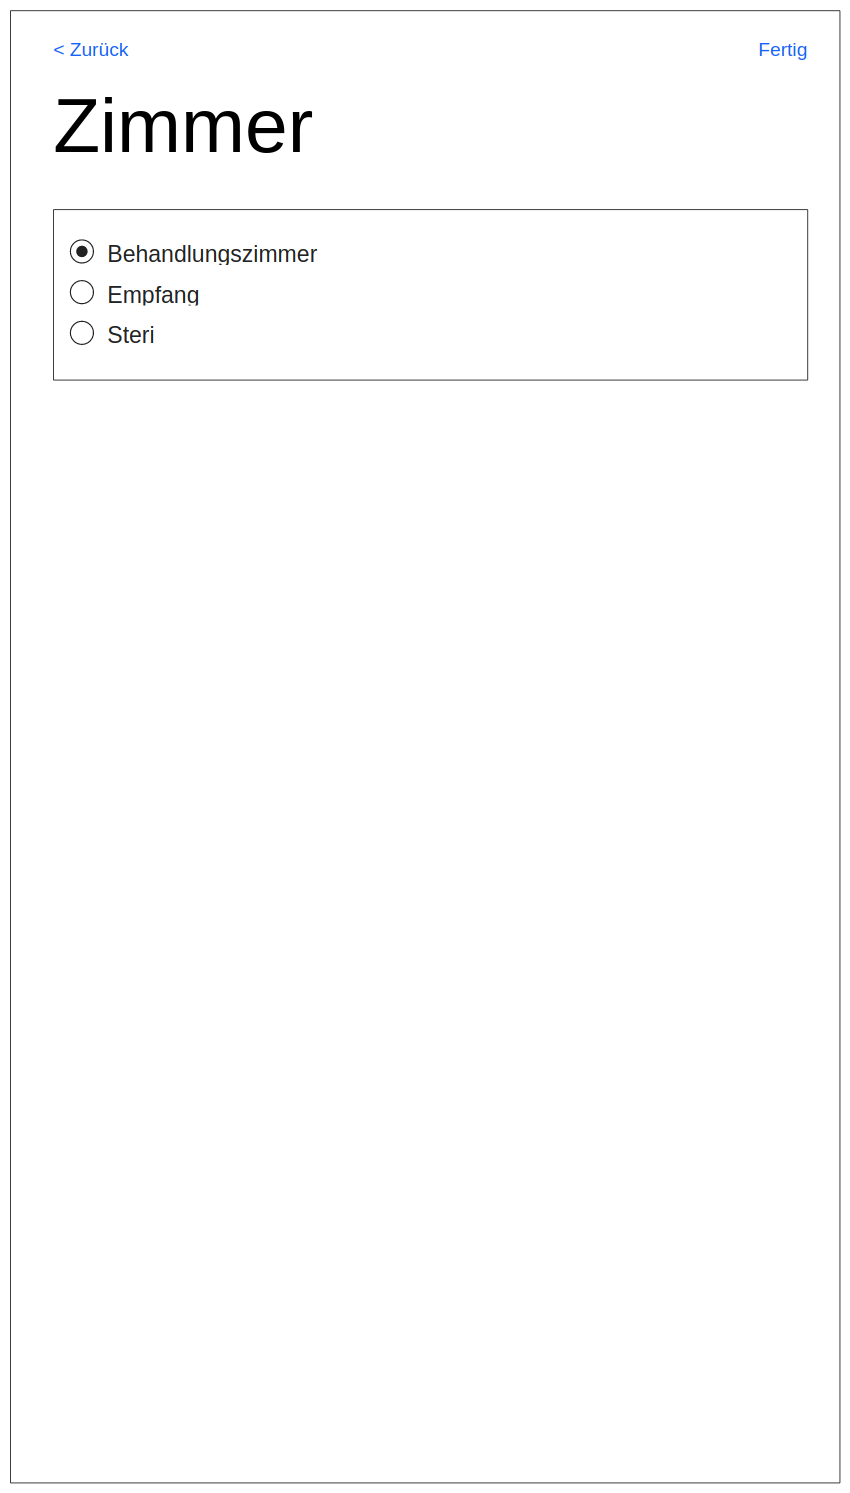
\includegraphics[width=\textwidth]{/home/joshua/FHNW/dev/IP6/IP6_Bachelorarbeit_Bericht_Cloudbasiertes_Praxisrufsystem/src/graphics/mockups/mockup_clientselect}
        \caption{Mockup Zimmerwahl}
    \end{minipage}\label{fig:Mockups-Login-ClientSelection}
\end{figure}

Die Zimmerauswahl besteht aus einem Seitentitel und einem Panel indem das gewünschte Zimmer ausgewählt werden kann.
In der Auswahl sind alle Zimmer zu sehen, welche dem Benutzer zur Verfügung stehen.
In der Kopfzeile sind die Schaltflächen ''Zurück'' und ''Fertig'' zu sehen.
Die Schaltfläche ''Zurück'', bricht die Anledung ab und führt zurück auf die Login Ansicht.
Die Schaltfläche ''Fertig'' bestätigt die Auswahl und leitet zur Hauptansicht weiter.
Wird bestätigt, ohne dass ein Zimmer angewählt ist, wird dem Benutzer eine Fehlermeldung angezeigt und nicht zur Hauptansicht weitergeleitet.

\clearpage

In der Hauptansicht gliedert sich in die Bereiche Home, Inbox und Einstellungen.
Zwischen den drei Bereichen kann über eine Leiste am unteren Ende des Bildschirms navigiert werden.
Die Ansicht Home zeigt dem Benutzer die Buttons, über welche er Meldungen versenden und Anrufe in der Gegensprechanlage starten kann.
Wird ein Anruf gestartet, wird die Ansicht für aktive Anrufe angezeigt.
Diese zeigt dem Benutzer den Titel des gestarteten Anrufs, sowie eine Liste aller Teilnehmer zusammen mit dem Verbindungsstatus jedes Teilnehmers.
Der Titel des Anrufes entspricht dem Anzeigetext des entsprechenden Buttons für ausgehende Anrufe und dem Namen des Anrufers für empfangene Anrufe.
Neben den Anrufinformationen zeigt die Ansicht für aktive Anrufe drei Buttons.
Über diese können Microfon und Lautsprecher des eigenen Gerätes stummgeschaltet werden.
Weiter kann über der Anruf über den dritten Button beendet werden.
Nach einem beendeten Anruf, wird zurück auf die Hauptansicht weitergeleitet.
Für den Anrufern ist das immer der Home Bereich.
Für den Empfänger entspricht es dem Bereich, der vor dem Empfang des Anrufes angezeigt wurde.

\begin{figure}[h]
    \centering
    \begin{minipage}[b]{0.4\textwidth}
        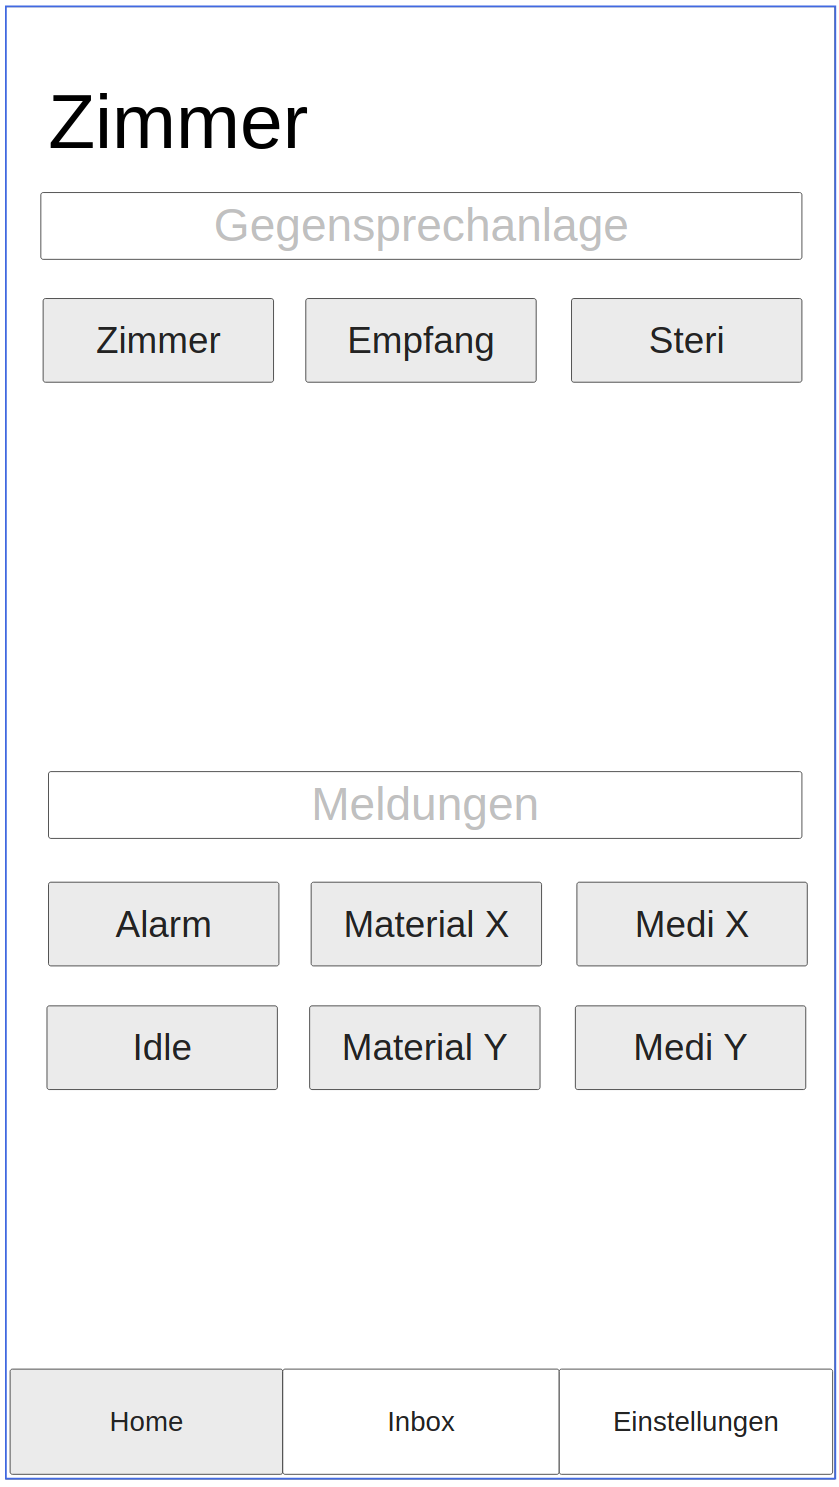
\includegraphics[width=\textwidth]{/home/joshua/FHNW/dev/IP6/IP6_Bachelorarbeit_Bericht_Cloudbasiertes_Praxisrufsystem/src/graphics/mockups/mockup_intercom}
        \caption{Mockup Home}
    \end{minipage}
    \hfill
    \begin{minipage}[b]{0.4\textwidth}
        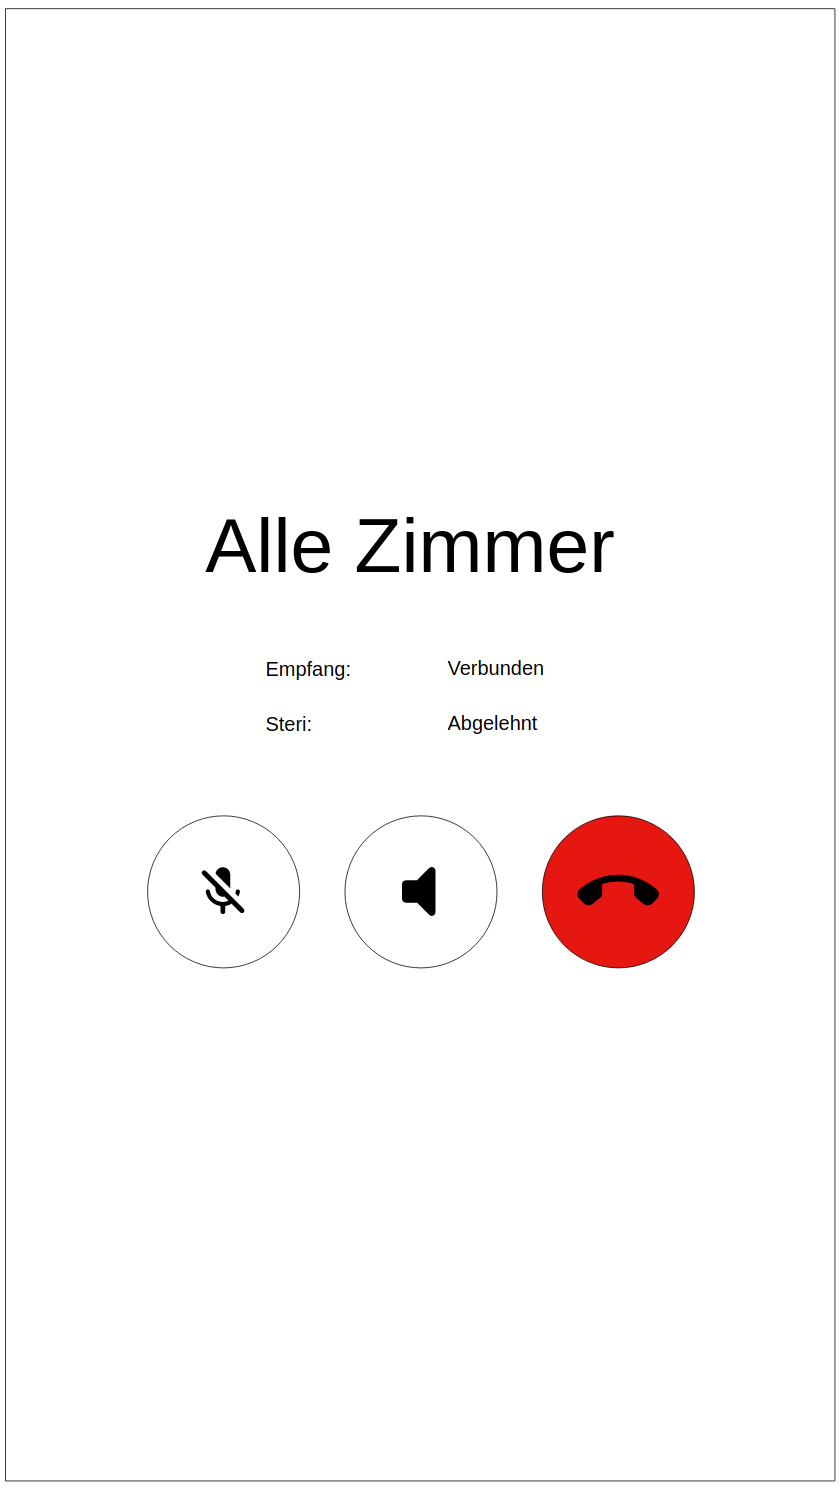
\includegraphics[width=\textwidth]{/home/joshua/FHNW/dev/IP6/IP6_Bachelorarbeit_Bericht_Cloudbasiertes_Praxisrufsystem/src/graphics/mockups/mockup_call}
        \caption{Mockup Aktiver Anruf}
    \end{minipage}\label{fig:Mockups-Home-ActiveCall}
\end{figure}

Der Bereich Inbox zeigt eine Liste der empfangenen Meldungen sowie der empfangenen und verpassten Anrufe.
Für Meldungen wird der Titel der Benachrichtigung gefolgt vom Namen des Versenders in Klammern sowie der Haupttext der Meldung angezeigt.
Für Anrufe wird der Name des Anrufers und ein Text der besagt ob es sich um einen empfangenen, verpassten oder abgelehnten Anruf handelt angezeigt.
Einträge für Meldungen sowie verpasste und abgelehnte Anrufe müssen durch antippen quittiert werden.
Solange unquittierte Meldungen oder Anrufe in der Inbox sind ertönt, wird im Abstand von 60 Sekunden eine Benachrichtigung angezeigt, die den Benutzer erinnert, die Inbox zu quittieren.
Der Bereich Settings zeigt den Namen des aktuellen Benutzers und ausgewählten Zimmers.
Über die Schaltfläche Abmelden, kann sich der Benutzer aus der Applikation abmelden.
Die Schaltfläche Benachrichtigungen vorlesen ist standardmässig aktiviert.
Wird die Option deaktiviert, werden Benachrichtigungen nie vorgelesen.
Die Schaltfläche Anruge empfangen ist ebenfalls standardmässig aktiviert.
Wird diese Option deaktiviert, werden alle empfangenen Anrufe automatisch abgelehnt und stattdessen eine Benachrichtigung angezeigt.
Ausgehende Anrufe können auch getätigt werden, wenn diese Option aktiviert ist.


\begin{figure}[h]
    \centering
    \begin{minipage}[b]{0.4\textwidth}
        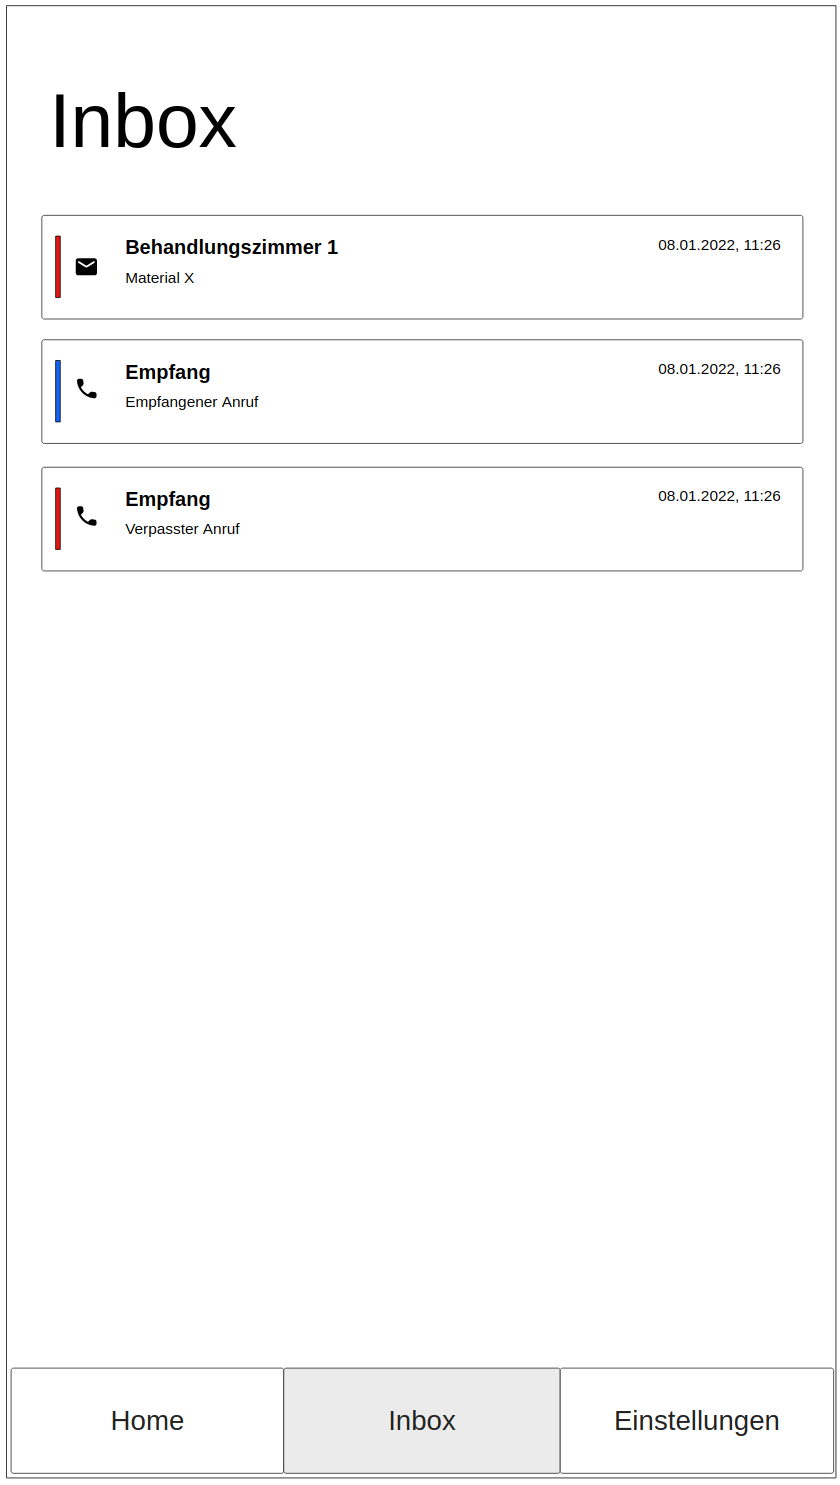
\includegraphics[width=\textwidth]{/home/joshua/FHNW/dev/IP6/IP6_Bachelorarbeit_Bericht_Cloudbasiertes_Praxisrufsystem/src/graphics/mockups/mockup_inbox}
        \caption{Mockup Inbox}
    \end{minipage}
    \hfill
    \begin{minipage}[b]{0.4\textwidth}
        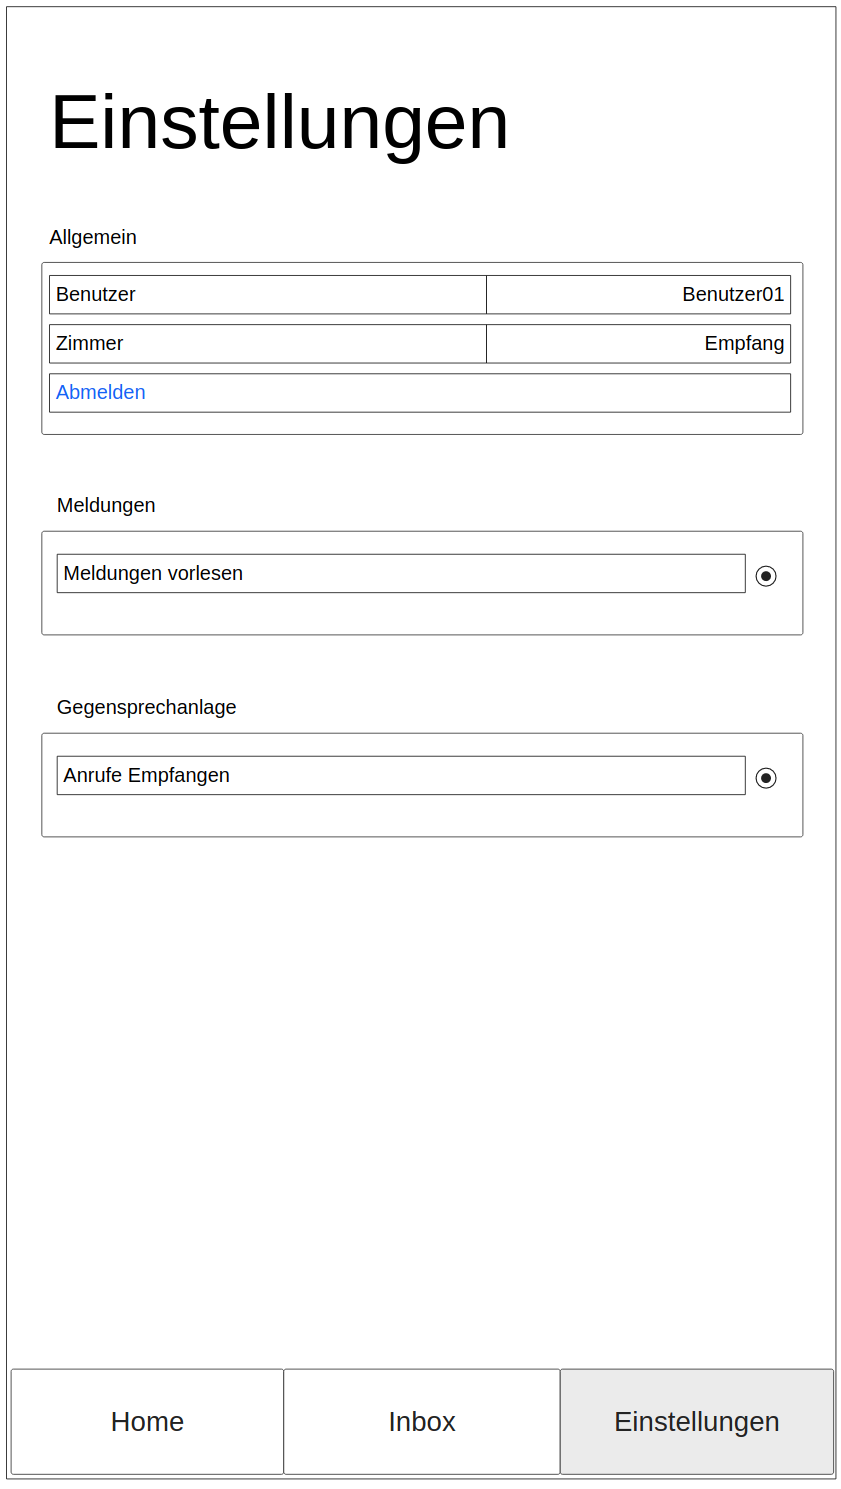
\includegraphics[width=\textwidth]{/home/joshua/FHNW/dev/IP6/IP6_Bachelorarbeit_Bericht_Cloudbasiertes_Praxisrufsystem/src/graphics/mockups/mockup_settings}
        \caption{Mockup Einstellungen}
    \end{minipage}\label{fig:Mockups-Inbox-Settings}
\end{figure}


\subsubsection{Anbindung Cloudservice}

Der Mobile Client muss an die API des Cloudservices angebunden werden.
Es wird eine Anbindung an die Domäne Configuration zur Anmeldung und Auswahl des gewünschten Zimmers, an die Domäne Notification zum Versenden von Benachrichtigungen und an die Domäne Speech Synthesis für den Bezug von Sprachdaten benötigt.
Die Schnittstellen dieser Domänen stehen als REST Endpoints zur verfügung.
In diesem Unterkapitel wird beschrieben, wie REST Aufrufe im nativen iOS Client integriert werden sollen.\footnote{Die Anbindung der Domäne Signaling findet nicht über REST statt und ist im Kapitel 5.2.4 beschrieben.}

Die Basisbibliothek für iOS Entwicklung bietet die Klasse URLSession, über welche Netzwerkaufrufe getätigt werden können.
Über URLSession.shared steht zudem eine Standard Instanz zur Verfügung, über welche Anfragen erstellt werden können.\cite{ios_urlsession}
Die Klasse UrlRequest ermöglicht es, Http-Request für eine URL mit Header und Body zu erstellen.\cite{ios_urlrequest}
Um die Integration dieser Klassen in den Mobile Client zu vereinfach, wird ein zentraler Service mit dem Namen PraxisrufApi erstellt.
Dieser kapselt das Erstellen, Befüllen und Absetzten der nötigen UrlRequest Instanzen und bietet öffentliche für die Http Verben Get, Post, Put und Delete an.




Beinhaltet Basisurl für Praxisurf API.
Parameter subUrl für spezifischen Ressourcen Pfad.
Parameter completion ist ein Callback für Result<T, PraxisrufApi>.
Result ist Klasse Basislibrary mit Typ für erfolgs und Fehlerfall.
Type für erfolgsfall ist generisch und wird vom Aufrufer mitgegeben.
Typ für Fehlerfall ist immer PraxisrufApi.g
Post und Put sollen zusätzlichen Parameter für RequestBody beinhalten.
API Service erstellt request aus URL, Methode und Body.
API Service setzt Authentication Header mit Bearer Token.
Das Token liest er dazu aus dem KeyStore.
Ist kein Token vorhanden, wird completion.fehlerfall mit noCredentials aufgerufen.
Andernfalls wird der Request abgesetzt.
Im Erfolgsfall wird der Body der Response nach T geparsed und completion.erfolg aufgerufen.
Im Fehlerfall wird completion.error aufgerufen.
Pro Domäne die angesprochen wird, wird eine Extionsionklasse erstellt.
Diese bietet Methoden mit sprechenden Namen für die angesprochene Funktionalität.
Die Methoden darin rufen die get, post, put und delete Methoden des API Service mit den entsprechenden Parametern auf.

Mit dieser Lösung steht ein Service zur verfügung, über welchen REST Calls einfach gemacht werden können.
Dank der generischen Methoden im Basis Service können neue Calls einfach hinzugefügt werden, ohne das Boilerplate Code wiederholt werden muss.
Durch die completion Methoden kann zudem jeder Call den Bedürfnissen des Aufrufers entsprechend abgehandelt werden.
Die Extension Klassen mit domänenspezifischen, sprechenden Methoden machen die verfügbaren Aufrufe übersichtlich.
Die API wird immer einheitlich über den generischen Service angesprochen.
Die Integration in den rest der Applikation über sprechende Namen führt dabei zu lesbarem und übersichtlicherem Code.

Der Service zur API Integration wird nicht direkt in den View Komponenten verwendet.
Es wird pro Domäne ein weiterer Service geschrieben, welche den Aufruf des API Services kapselt.
Dieser Service bietet Methoden, über welche der API Service angesprochen werden kann.
Die Methoden des Integration Services nehmen die Informationen, welche aus der Benutzeroberfläche Stammen als Parameter entgegen.
Alle weiteren Informationen welche für den API Aufruf nötig sind, werden im Integration Service geladen.
Dies beinhaltet Credentials, welche aus dem KeyStore geladen werden sowie die Daten der aktuell aktiven Client Configuration, welche aus den UserDefaults geladen werden.

Die Integration Services werden als ObservableObjects implementiert.
Die Resultate der API Calls werden im Service als Instanzvariable mit @Published gesetzt.
Die View, welche einen Integration Service verwendet, kann Bindings auf diese @Published Resultate setzten.

\subsubsection{Anbindung Messaging Service}

Als Messaging Service wird Firebase Cloud Messaging verwendet.
Firebase bietet eine native library mit welcher Firebase Cloud Messaging in iOS Clients integriert werden kann.
Diese Integration kann allerdings nicht mit dem Mitteln von SwiftUI implementiert werden.
Dies liegt daran, dass für das Empfangen von Benachrichtigungen und das Anzeigen von Push Benachrichtigungen Integration mit dem Betriebsystem notwendig ist.
Diese Integration kann bis heute nur über AppDelegates aus der UIKit Welt umgesetzt werden.
SwiftUI Applikationen können oft ohne AppDelegates implementiert werden.
Sobald aber Integration mit dem Betriebsystem notwendig ist, müssen AppDelegates verwendet werden.
Dazu können AppDelegates bei der Initialisierung der Applikation registriert werden.

Zur Anbindung von Firebase Cloud Messaging an den Mobile Client wird dementsprechend ein AppDelegate implementiert.
In diesem AppDelegate müssen vier Funktionen implementiert werden:

\begin{enumerate}
    \item Beim Start der Applikation muss sich der Mobile Client beim Messaging Service registrieren.
    \item Das Token, welches den Client beim Messaging Service identifiziert wird regelmässig erneuert. Der App Delegate muss darauf reagieren und das erneuerte Token an die Applikation übergeben.
    \item Benachrichtigungen die im Vordergrund empfangen werden, müssen als Push Benachrichtigugn angezeigt werden und an die Applikation übergeben werden.
    \item Benachrichtigungen die im Hintergrund empfangen werden, müssen angezeigt werden.
    \item Sobald die Applikation wieder in den Vordergrund tritt, müssen im Hintergrund empfangene Benachrichtigungen der Applikation übergeben werden.
    \item Wenn er Client sich abmeldet muss die Registrierung beim Messaging Service entfernt werden. Dies geschieht ebenfalls im AppDelegate.
\end{enumerate}




Die Anbindung erfolgt damit wie in der offiziellen Dokumentation vorgesehen.
Damit die Abhängigkeit zu AppDelegates minimiert ist, sollen innerhalb der AppDelegates nur minimale Logik ausgeführt werden.
Die echte Logik wird an unabhängige Services delegiert.


\subsubsection{Anbindung Singaling}

Lorem Ipsum\\

\subsubsection{Integration WebRTC}

Lorem Ipsum\\


\subsubsectio{Scheduled Reminder für Inbox}
IOS Development unterstützt scheduled tasks.

\clearpage
